\documentclass{article}


\usepackage[utf8]{inputenc}
\usepackage{amsthm}
\usepackage{amssymb}
\usepackage{amsfonts}
\usepackage[francais]{babel}
\usepackage{fancyvrb}
\usepackage{hyperref}
\usepackage{graphicx}
\usepackage{listings}

\author{Ye Daniel, Kouadri Amine.} 

\title{Compte-rendu du TP4}

\begin{document}

\maketitle Notre code est constitué des fichiers "Prime.py", "factorisation.py", bezout.py", et "rsa.py".
Voici les réponses aux questions du tp (hors programmation):
\paragraph{question 1.a:}
~~\\
\\ 
On obtient le quotient de la division de a par b avec "a/b", quant au reste il s'obtient en codant comme suit, "a\%b".
\paragraph{question 1.b:}
~~\\
\\ 
Un nombre premier est un nombre qui n'est divisible que par lui-même et par 1. 2 est le premier nombre premier, et le seul nombre premier paire.
\paragraph{question 1.c:}
~~\\
\\ 
Une méthode pour savoir si un nombre est premier ou non est de voir si il est divisible par tous les nombres inférieurs à sa racine carrée.
1001 est divisible par 7, il n'est pas premier.
89999 est divisible par 7, il n'est pas premier.
2017 3001 et 49999 sont premiers.
\paragraph{question 1.d:}
~~\\
\\ 
Les nombres de Fermat sont les nombres de la forme $F_n=2^{2^{n}}+1$
\\
Voici les 5 premiers nombres de Fermat:
$F_0=3$,
$F_1=5$,
$F_2=17$,
$F_3=257$,
$F_4=65537$,
les 4 premiers nombres sont bien premiers.
$F_5=4294967297$.
\\
\\
Le mathématicien Euler a démontré que tout diviseur premier de $F_n$ est de la forme:
$p=k\times2^{n+1}+1$
En prenant $k=10$ on trouve bien un nombre premier qui divise F5. On a $p=641$.
Le quotient de cette division est 6700417. On a $F5=641\times6700417$ et par conséquent F5 n'est pas premier.

\paragraph{question 2.a:}
~~\\
\\
On considère tous les nombres inférieurs à n. Le crible d'Erathosène consiste à procéder par élimination en supprimant tous les multiples de 2 ensuite tous les multiples des nombres restants. L'algorithme s'arrête lorsque le carrée du premier nombre restant est supérieur au dernier nombre restant.(C'est-à-dire lorsque le plus petit nombre restant est supérieur à la racine carrée du plus grand nombre restant.)
\\
\\
Voici la liste des nombres premiers inférieurs à 200:
\\
2, 3, 5, 7, 11, 13, 17, 19, 23, 29, 31, 37, 41, 43, 47, 53, 59, 61, 67, 71, 73, 79,\\ 83, 89, 97, 101, 103, 107, 109, 113, 127, 131, 137, 139, 149, 151, 157, 163,\\ 167, 173, 179, 181, 191, 193, 197, 199

\paragraph{question 2.c:}
~~\\
\\
Voici le contenu du fichier txt qui comprend tous les nombres premiers inférieurs à 1000:
\lstinputlisting[language=bash]{primes.txt}

\paragraph{question 2.d:}
~~\\
\\
Soit $\pi(n)$ le nombre de nombres premiers inférieurs à n. Voici le graphique de $\pi(n)$ en fonction de n, pour n variant de 2 à 1000, ainsi que la fonction $f(n)=\frac{n}{log(n)}$:
\\
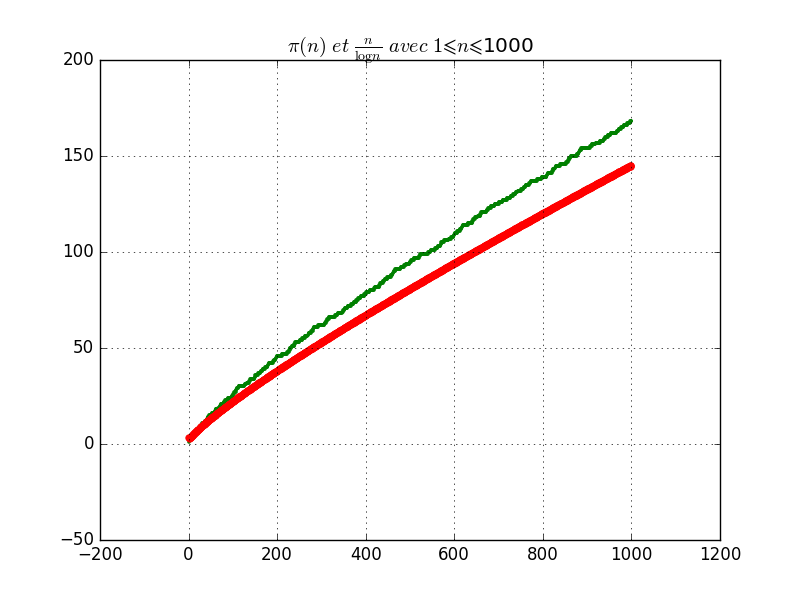
\includegraphics[height=8cm]{n_1000.png}
\\
On a $\lim\limits_{x \rightarrow +\infty} \pi(x)\frac{log(x)}{x}=1$
\\
C'est-à-dire que les fonctions $\pi(x)$ et $\frac{n}{log(n)}$ sont équivalentes lorsque x tend vers $\infty$.
\paragraph{question 2.e:}
~~\\
\\
Voici le fichier txt qui donne $\pi(n)$, $\frac{n}{log(n)}$, pour $n=10^{k}$, k variant de 1 à 6.
\lstinputlisting[language=bash]{table.txt}
\paragraph{question 3.a:}
~~\\
\\
Le théorème fondamental de l'arithmétique s'énonce ainsi: Tout nombre s'écrit de façon unique comme un produit de facteurs premiers.
\paragraph{question 3.b:}
~~\\
\\
$924=2^{2}\times3\times7\times11$
\paragraph{question 4.a:}
~~\\
\\
Le PGCD de deux nombres est le plus grand diviseur commun aux deux nombres.
\paragraph{question 4.b:}
~~\\
\\
On compare les décompositions en facteurs premiers des deux nombres, on prend les nombres communs à ces décompositions élevés à la plus petite puissance du nombre retrouvée dans les décompositions.
Par exemple, pour 4864 et 3458. On a:
\\
$4864=2^{8}\times19$
\\
$3458=2\times7\times13\times19$
\\
Le PGCD de ces deux nombres est égal à $2\times19$, c'est-à-dire 38.
\\
On peut aussi retrouver le PGCD avec la méthode d'Euclide dite des divisions successives. (Nous avons utilisé les deux méthodes présentes dans le fichier "bezout.py")
\paragraph{question 4.c:}
~~\\
\\
Identité de Bézout: soit a et b deux entiers naturels et d leur PGCD. Il existe deux entiers relatifs x et y tels que $ax+by=d$.
\paragraph{question 4.d:}
~~\\
\\
Avec l'algorithme d'Euclide étendu on obtient, pour a=4864 et b=3458, d=38, x=32 et y=-45.
\end{document}